% $Id: jets-and-algs.tex 472 2019-01-18 12:07:31Z smarzani $ 
%
% Descriptino of what jets are and what algoriotyhms are used to
% reconstruct them
%------------------------------------------------------------------------
\chapter{Jets and jet algorithms}\label{chap:jets-and-algs}

\section{The concept of jets}\label{sec:jet-concept}

When studying high-energy collisions one often has to consider
processes where quarks and gluons are produced in the final-state.
%
For $e^+e^-$ collisions, the study of hadronic final-states has been a
major source of information, helping to establish QCD as the
fundamental theory of strong interactions, but also providing a clean
playground for the study of perturbative QCD and the tuning of
Monte-Carlo event generators.
%
At the LHC, the list of processes involving high-energy quarks and/or
gluons in their final state is even longer. First, since we collide
protons, a hard QCD parton can be radiate from the incoming
partons. Then, other particles like W, Z and Higgs bosons can
themselves decay to quarks. And, finally, when searching for new
particles, one often has to consider decay chains involving quarks and
gluons.

However, these high-energy quarks and gluons are not directly observed
in the final state of the collision. First of all, as mentioned in the
previous chapters, they tend to undergo successive branchings at small
angles, producing a series of collimated quarks and gluons. The fact that this parton shower is
collimated traces back to the collinear divergence of QCD.
%
Starting from a parton with high virtuality (of the order of the hard
scale of the process), the parton shower will produce branchings into
further partons of decreasing virtuality, until one reaches a
non-perturbative (hadronisation) scale, typically of order
$\Lambda_\text{QCD}$ or $1$~GeV.
%
At this stage, due to confinement, these quarks and gluons will form
hadrons. Although some analytic approaches to hadronisation exist,
this non-perturbative step often relies on models implemented in Monte
Carlo Event generators.

Overall, the high-energy partons produced by the collision appear in
the final state as a collimated bunch of hadrons that we call {\em
  jets}.
%
Conceptually, {\it jets are collimated flows of hadrons and they can
  be seen as proxies to the high-energy quarks and gluons produced in
  a collision}.
%
This behaviour is observed directly in experiments where the hadronic
final state appears to be collimated around a few directions in the
detector.


\subsection{Jet definitions and algorithms}\label{sec:jet-algs}

The above picture is over-simplified in a few respects.
%
First of all, partons are ill-defined objects, \eg due to
higher-order QCD corrections where additional partons, real or
virtual, have to be included.
%
Then, whether two particles are part of the same jet or belong to two
separate jets also has some degree of arbitrariness, related to what
we practically mean by ``collimated''. 

The simple concept of what a jet is meant to represent is therefore
not sufficient to practically identify the jets in an event.
%
To do that, one relies on a {\em jet definition}, \ie a well-defined
procedure that tells how to reconstruct the jets from the set of
hadrons in the final state of the collision.

A jet definition can be seen as made of a few essential building
blocks: the {\em jet algorithm}, which is the recipe itself and a set
of parameters associated with free knobs in the algorithm. A typical
parameter, present in almost all jet definitions used in hadron
colliders is the {\em jet radius} which essentially provides a
distance in the rapidity-azimuth ($y-\phi$) plane above which two
particles are considered as no longer part of the same jet, \ie no
longer considered as collinear.

In addition, a jet definition uses a {\em recombination scheme} which
specifies how the kinematic properties of the jet are obtained from
its constituents.
%
Most applications today use the {\em ``$E$-scheme''} recombination
scheme which simply sums the components of the four-vectors. Other
recombination schemes, like the massless $p_t$ or $E_t$ schemes, have
been used in the past but are not discussed here.
%
Several jet-substructure applications make use of the {\em
  winner-take-all} (WTA) recombination scheme \cite{Larkoski:2014uqa}
where the result of the recombination of two particles has the
rapidity, azimuth and mass of the particle with the larger $p_t$, and
a $p_t$ equal to the sum of the two $p_t$'s. As we will further
discuss later in this book, this approach has the advantage that
it reduces effects related to the recoil of the jet axis when
computing jet observables that share similarities with the event-shape broadening~\cite{Rakow:1981qn}.

Over the past few decades, a number of jet algorithms have been
proposed. They typically fall under two big categories: {\em cone
  algorithms} and {\em sequential-recombination algorithms}. We
discuss them both separately below, focusing on the algorithms that
have been most commonly used recently at hadronic colliders.
%
For an extensive review on jet definitions, we highly recommend the
reading of Ref.~\cite{Salam:2009jx}.

\subsection{Basic requirements}\label{sec:jetalgs-snowmass}

Before giving explicit descriptions of how the most commonly-used jet
algorithms are defined, we briefly discuss what basic properties we do
expect them to satisfy.
%
In the 1990s a group of theorists and Tevatron experimentalists
formulated what is known as the Snowmass accord~\cite{Huth:1990mi}. This document
listed the fundamental criteria that any jet algorithm should
satisfy.

\vspace*{0.3cm}\noindent\centerline{\fbox{
\begin{minipage}{0.9\textwidth}
%\sf 
Several important properties that should be met by a jet definition are:
\vspace*{-0.2cm}
\begin{enumerate}
  \itemsep-0.1cm
\item Simple to implement in an experimental analysis;
\item Simple to implement in the theoretical calculation;
\item Defined at any order of perturbation theory;
\item Yields finite cross sections at any order of perturbation theory;
\item Yields a cross section that is relatively insensitive to hadronisation.
\end{enumerate}
\end{minipage}
}}\vspace*{0.3cm}

The first two criteria are mostly practical aspects. For example, if
an algorithm is too slow at reconstructing jets in an experimental
context, it would be deemed impractical. These two conditions also
mean that the algorithm should be applicable to an input made either
of partons (in a theoretical calculation), or of tracks and
calorimeter towers (in an experiment analysis).
%
The third and fourth conditions are mainly those of
IRC safety, a requirement that, as we have already seen, is at the core of
perturbative QCD calculations.
%
The fifth condition is a little bit more subjective.  We have already
seen that the description of a particle-collision event relies upon
several building blocks: the short-distance interaction computed in
fixed-order perturbation theory, the parton shower, the hadronisation
process and multi-parton interactions.
%
Since jets are supposed to capture the ``hard partons in an event'',
one should hope that the jets which come out of each of these
different steps of an event simulation are in good agreement. In
particular, this means that observables built from jet quantities
should be as little sensitive as possible to non-perturbative effects
like hadronisation and the Underlying Event.
%
Furthermore, to be simple to implement in an experimental analysis,
the jets should also be as little sensitive as possible to detector
effects and pileup.

The question of the sensitivity of different jet definitions to
non-perturbative effects, pileup and detector effects has been an
active topic of discussion when deciding which algorithm to use at
Tevatron and the LHC. A complete assessment of this question is
clearly beyond the scope of the present lecture notes. We will however
come back to a few crucial points when introducing the different
relevant jet definitions below.


\section{Sequential recombination algorithms}\label{sec:jetalgs-recombination}

Sequential recombination algorithms are based on the concept that,
from a perturbative QCD viewpoint, jets are the product of successive
parton branchings. These algorithms therefore try to invert this
process by successively recombining two particles into one. This
recombination is based on a distance measure that is small when the
QCD branching process is kinematically enhanced. Thus, one
successively recombine particles which minimise the distance in order
to mimic the QCD dynamics of the parton shower.
%
It is easy to check that all the recombination algorithms described
below are infrared-and-collinear safe.

\paragraph{Generalised-$k_t$ algorithm.}
%
Most of the recombination algorithms used in the context of hadronic
collisions belong to the family of the {\em generalised-$k_t$
  algorithm}~\cite{Cacciari:2011ma} which clusters jets as follows.
\begin{enumerate}
\item Take the particles in the event as our initial list of objects.
\item From the list of objects, build two sets of distances: an
  {\em inter-particle distance}
  \begin{equation}
    d_{ij} = \text{min}(p_{t,i}^{2p},p_{t,j}^{2p})\Delta R_{ij}^2,
  \end{equation}
  where $p$ is a free parameter and $\Delta R_{ij}$ is the geometric
  distance in the rapidity-azimuthal angle plane
  (Eq.~(\ref{eq:DeltaR-def}), and a {\em beam distance}
  \begin{equation}
    d_{iB} = p_{t,i}^{2p}R^2,
  \end{equation}
  with $R$ a free parameter usually called the {\em jet radius}.
\item Iteratively find the smallest distance among all the
  $d_{ij}$ and $d_{iB}$
  \begin{itemize}
  \item If the smallest distance is a $d_{ij}$ then objects $i$ and
    $j$ are removed from the list and recombined into a new object $k$
    (using the recombination scheme) which is itself added to the
    list.
  \item If the smallest is a $d_{iB}$, object $i$ is called a {\em
      jet} and removed from the list.
  \end{itemize}
  Go back to step 2 until all the objects in the list have
  been exhausted.
\end{enumerate}

In all cases, we see that if two objects are close in the
rapidity-azimuth plane, as would be the case after a collinear parton
splitting, the distance $d_{ij}$ becomes small and the two objects are
more likely to recombine. Similarly, when the inter-particle distances
are such that $\Delta R_{ij}>R$, the beam distance becomes smaller
than the inter-particle distance and objects are no longer recombined,
making $R$ a typical measure of the size of the jet.

\paragraph{$k_t$ algorithm.}
%
Historically, the best-known algorithm in the generalised-$k_t$ family
is the {\em $k_t$ algorithm}~\cite{Catani:1993hr,Ellis:1993tq},
corresponding to $p=1$ above. In that case, a soft emission, \ie one
with small $p_t$, would also be associated a small distance and
therefore recombine early in the clustering process. This is
motivated by the fact that soft emissions are also enhanced in
perturbative QCD.\footnote{Note that the presence of the ``min'' in
  the distance measure, instead of a product, guarantees that two soft
  objects far apart are not recombined. This would lead to undesired
  behaviours and complex analytic structures, as it is the case with
  the JADE algorithm~\cite{Bartel:1986ua,Bethke:1988zc}.}
%
Its sensitivity to soft emissions, while desirable from a perturbative
QCD standpoint, has the disadvantage that jets become more sensitive
to extra soft radiation in the event, typically like the Underlying
Event or pileup.
%
Although the Tevatron experiments have sometimes resorted to the $k_t$
algorithm, they have predominantly used cone algorithms (see below)
for that reason.

\paragraph{Cambridge/Aachen algorithm.}
Another specific cases of the generalised-$k_t$ algorithm is the {\em
  Cambridge/Aachen algorithm}~\cite{Dokshitzer:1997in,Wobisch:1998wt},
obtained by setting $p=0$ above.
%
In this case, the distance becomes purely geometrical and suffers less
from the contamination due to soft backgrounds than the $k_t$
algorithm does.

\paragraph{Anti-$k_t$ algorithm.}
In the context of LHC physics, jets are almost always reconstructed
with the {\em anti-$k_t$ algorithm}~\cite{Cacciari:2008gp}, which
corresponds to the generalised-$k_t$ algorithm with $p=-1$. The
primary advantage of this choice is that it favours hard particles
which will cluster first.
%
A hard jet will grow by successively aggregating soft particles around
it until it has reached a (geometrical) distance $R$ away from the jet
axis. This means that hard jets will be insensitive to soft radiation
and have a circular shape in the $y-\phi$ plane.
% 
This soft-resilience of the anti-$k_t$ algorithm largely
facilitates its calibration in an experimental context and is the main
reason why it was adopted as the default jet clustering algorithm by
all the LHC experiments.

\begin{figure}
  \centering
  \raisebox{1.8cm}{\phantom{$\!\to\!$}}{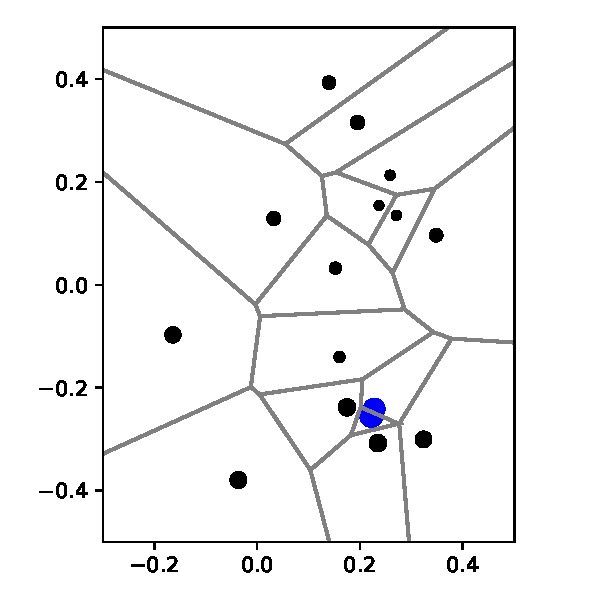
\includegraphics[width=0.24\textwidth,page=1]{figures/jet-clustering-cartoon.pdf}}%
  \raisebox{1.8cm}{$\!\!\to$}{\includegraphics[width=0.24\textwidth,page=2]{figures/jet-clustering-cartoon.pdf}}%
  \raisebox{1.8cm}{$\!\!\to$}{\includegraphics[width=0.24\textwidth,page=3]{figures/jet-clustering-cartoon.pdf}}%
  \raisebox{1.8cm}{$\!\!\to$}{\includegraphics[width=0.24\textwidth,page=4]{figures/jet-clustering-cartoon.pdf}}\\
  \raisebox{1.8cm}{$\!\!\to$}{\includegraphics[width=0.24\textwidth,page=5]{figures/jet-clustering-cartoon.pdf}}%
  \raisebox{1.8cm}{$\!\!\to$}{\includegraphics[width=0.24\textwidth,page=6]{figures/jet-clustering-cartoon.pdf}}%
  \raisebox{1.8cm}{$\!\!\to$}{\includegraphics[width=0.24\textwidth,page=7]{figures/jet-clustering-cartoon.pdf}}%
  \raisebox{1.8cm}{$\!\!\to$}{\includegraphics[width=0.24\textwidth,page=8]{figures/jet-clustering-cartoon.pdf}}\\
  \raisebox{1.8cm}{$\!\!\to$}{\includegraphics[width=0.24\textwidth,page=9]{figures/jet-clustering-cartoon.pdf}}%
  \raisebox{1.8cm}{$\!\!\to$}{\includegraphics[width=0.24\textwidth,page=10]{figures/jet-clustering-cartoon.pdf}}%
  \raisebox{1.8cm}{$\!\!\to$}{\includegraphics[width=0.24\textwidth,page=11]{figures/jet-clustering-cartoon.pdf}}%
  \raisebox{1.8cm}{$\!\!\to$}{\includegraphics[width=0.24\textwidth,page=12]{figures/jet-clustering-cartoon.pdf}}\\
  \raisebox{1.8cm}{$\!\!\to$}{\includegraphics[width=0.24\textwidth,page=13]{figures/jet-clustering-cartoon.pdf}}%
  \raisebox{1.8cm}{$\!\!\to$}{\includegraphics[width=0.24\textwidth,page=14]{figures/jet-clustering-cartoon.pdf}}%
  \raisebox{1.8cm}{$\!\!\to$}{\includegraphics[width=0.24\textwidth,page=15]{figures/jet-clustering-cartoon.pdf}}%
  \raisebox{1.8cm}{$\!\!\to$}{\includegraphics[width=0.24\textwidth,page=16]{figures/jet-clustering-cartoon.pdf}}
  % 
  \caption{
    Illustration of a step-by-step clustering using the anti-$k_t$
    algorithm with $R=0.4$.
    %
    The axes of each plot are rapidity and azimuthal angle. 
    %
    Each particle is represented by a cross with a size increasing
    with the $p_t$ of the particle.
    %
    To help viewing the event, we also draw in grey lines the Voronoi
    cells obtained for the set of particles in the event (\ie cells
    obtained from the bisectors of any pair of points).
    %
    Each panel corresponds to one step of the clustering.
    %
    At each step, the dots represent the objects which are left 
    for clustering (again, with size increasing with $p_t$).
    %
    Pairwise clusterings are indicated by a blue pair of dots, while
    red dots correspond to final jets (\ie beam clusterings).
    %
    The shaded areas show the cells included in each of the three jets
    which are found ultimately. 
    %
  }\label{fig:jet-clustering-steps}
\end{figure}

\begin{figure}
  \centering
  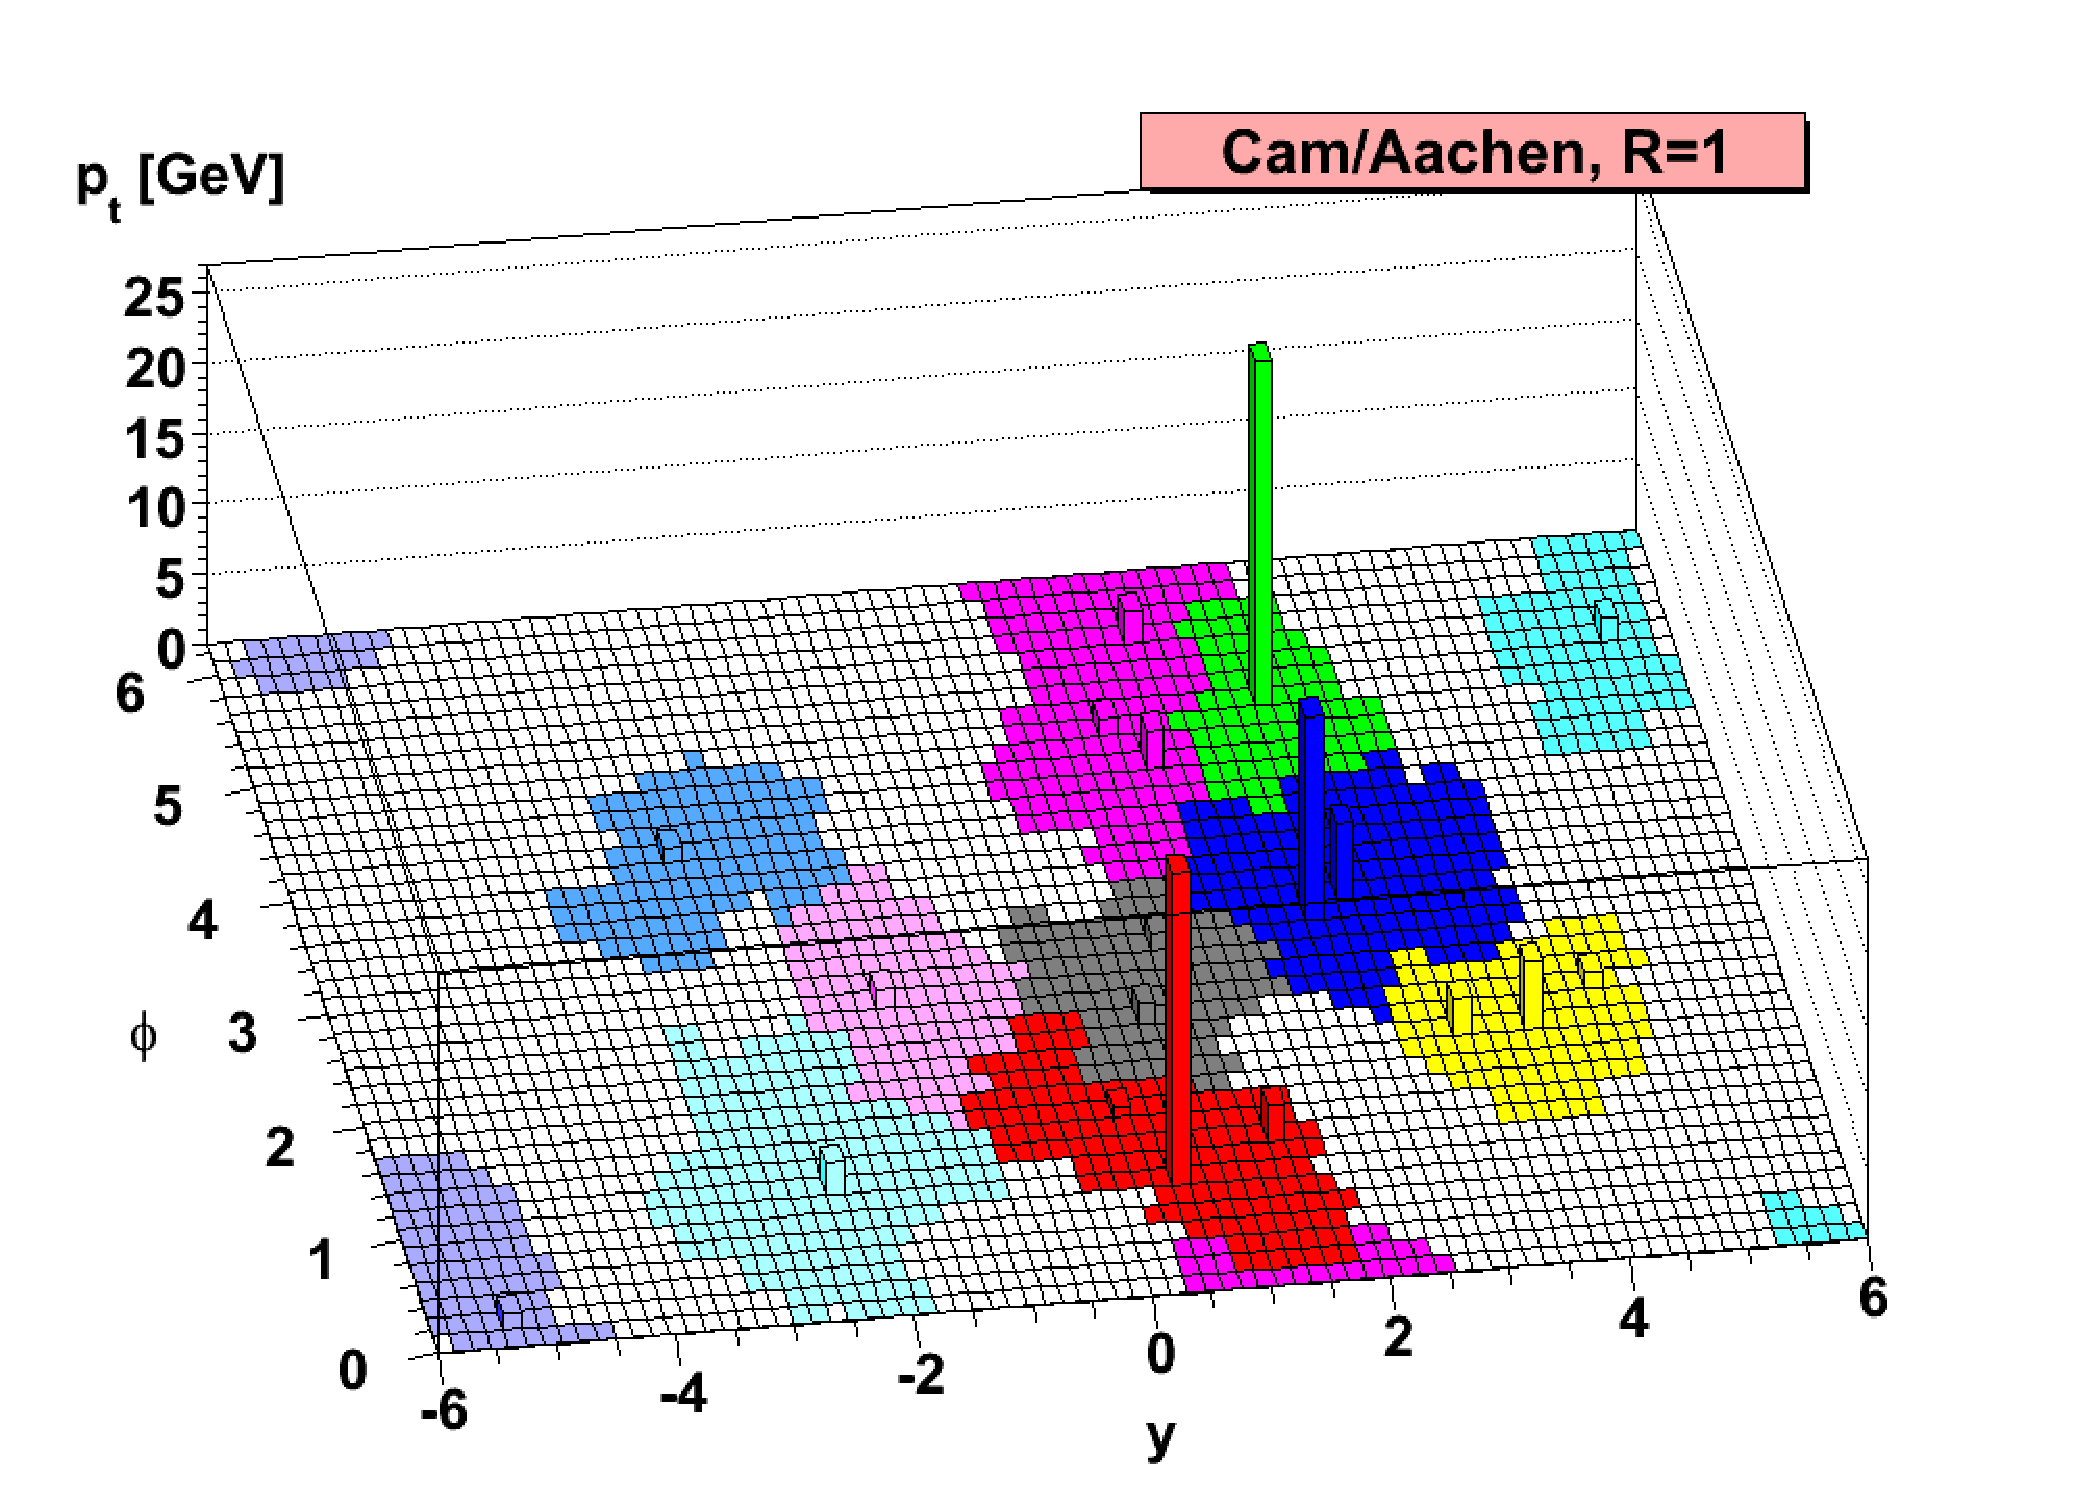
\includegraphics[width=0.48\textwidth]{figures/event-root-active-cam.pdf}%
  \hfill%
  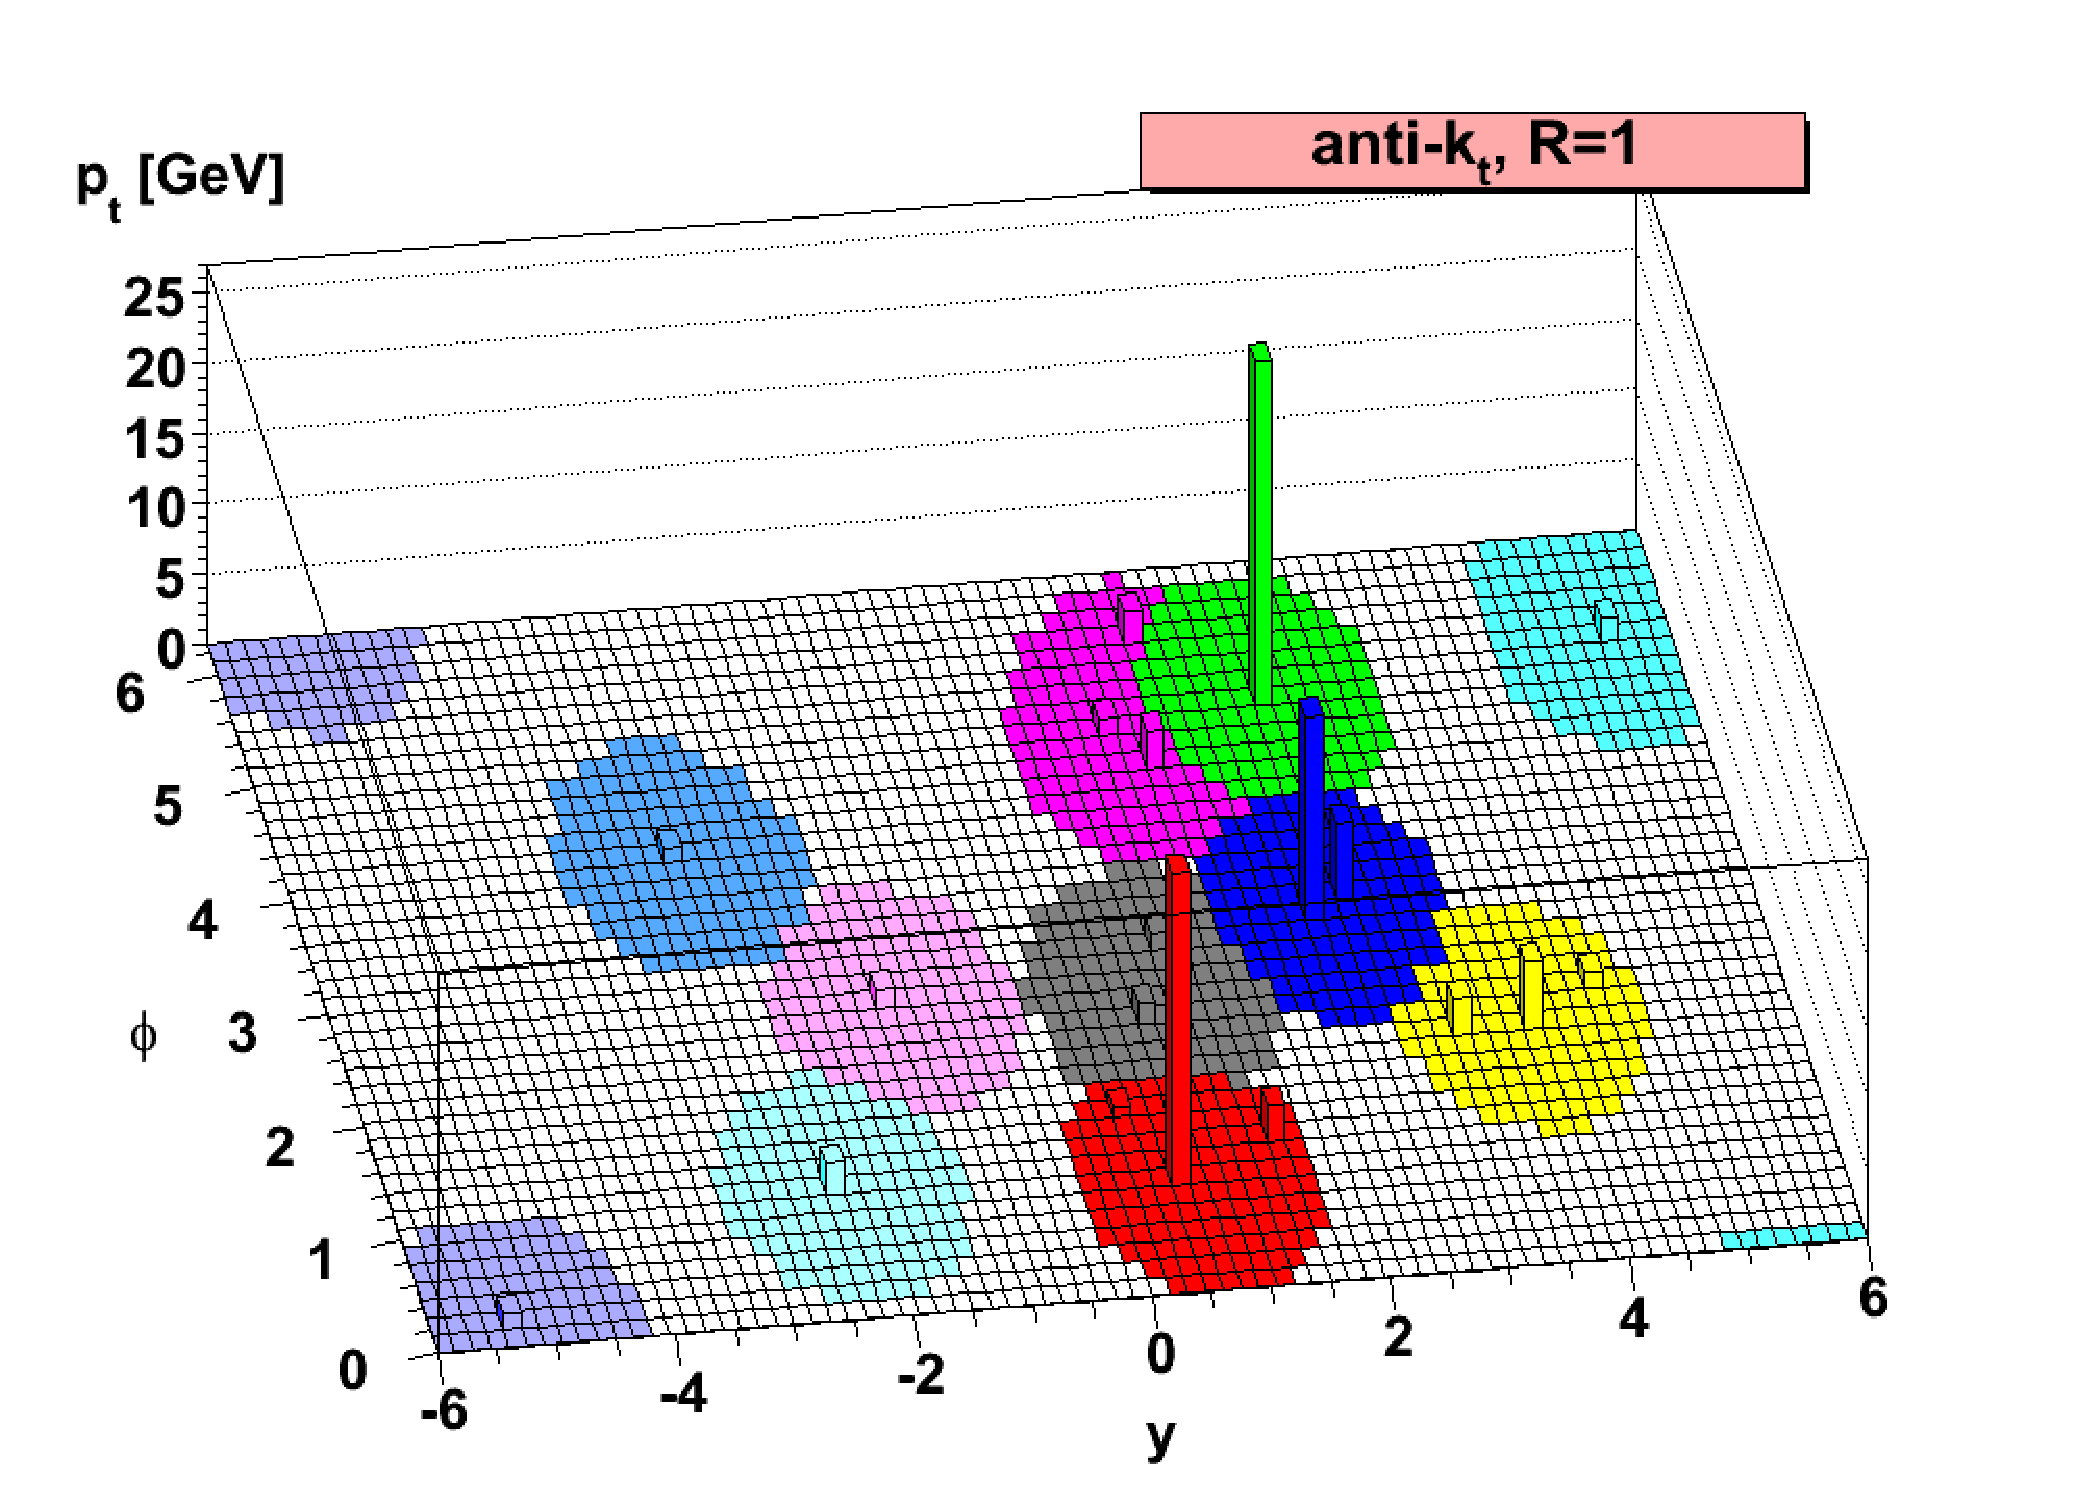
\includegraphics[width=0.48\textwidth]{figures/event-root-active-antikt.pdf}  
  \caption{Jets obtained with the Cambridge/Aachen (left) and
    anti-$k_t$ (right) algorithms with $R=1$. The shaded regions
    correspond to the (active) catchment
    area~(see~\cite{Cacciari:2008gn}) of each jet. While the jets
    obtained with the Cambridge/Aachen algorithm have complex
    boundaries (a similar property would be seen on $k_t$ jets), the
    hard jets obtained with anti-$k_t$ clustering are almost
    perfectly circular. This figure has been taken from~\cite{Cacciari:2008gp}.}\label{fig:jet-areas}
\end{figure}

To make things more concrete, we show in
Fig.~\ref{fig:jet-clustering-steps} a step-by-step example of a
clustering sequence with the anti-$k_t$ jet algorithm on a small set
of particles.
%
The successive pairwise recombinations, and beam recombination
giving the final jets, is clearly visible on this figure.
%
Finally, the resilience of anti-$k_t$ jets with respect to soft radiation is shown
in Fig.~\ref{fig:jet-areas}, where we see that anti-$k_t$ jets have a
circular shape while Cambridge/Aachen jets have complex
boundaries.\footnote{In practice, the jet areas are obtained by adding
  a infinitely soft particles, {\em aka} ghosts, to each calorimeter
  tower, These are clustered with the hard jets, indicating the
  boundaries of the jets.}

\paragraph{Relevance for jet substructure.}
%
In the context of jet substructure studies, several recombination
algorithms are used. Initially, jets are usually reconstructed using
the anti-$k_t$ algorithm with a large radius (typically $R$ in the
0.8--1.2 range). Many substructure tools then rely on reclustering the
constituents of that jet with another sequential-recombination jet
algorithm (or jet definition), allowing one to have a convenient view
of the jet clustering as a tree structure.
%
The most commonly used algorithm is probably Cambridge/Aachen since it
gives a natural handle on the structure of the jet at different
angular scales, in a way that respects the angular ordering of parton
showers (see.\ also~\cite{Dreyer:2018nbf}).
%
One also relies on the $k_t$ algorithm used \eg to split the jet into
subjets, or the generalised-$k_t$ algorithm with $p=1/2$, used because
it mimics an mass/virtuality ordering of the subjets.
%
More details will be given later when we review the main substructure
tools.

\section{Cone algorithms}\label{sec:jetalgs-cone}

Cone algorithms were first introduced in
1979~\cite{Sterman:1977wj}. They are based on the
idea that jets represent dominant flows of energy in an event.
%
Modern cone algorithms rely on the concept of a {\em
  stable cone}: for a given cone centre $y_c,\phi_c$ in the
rapidity-azimuth plane, one sums the 4-momenta of all the particles
with rapidity and $\phi$ within a (fixed) radius $R$ around the cone
centre; if the 4-momentum of the sum has rapidity $y_c$ and
azimuth $\phi_c$ --- \ie the sum of all the momenta in the cone points
in the direction of the centre of the cone --- the cone is called {\em
  stable}.
%
This can be viewed as a self-consistency criterion.

In order to find stable cones, the JetClu~\cite{Abe:1991ui} and
(various) midpoint-type~\cite{Blazey:2000qt,Abazov:2011vi} cone
algorithms use a procedure that starts with a given set of
seeds. Taking each of them as a candidate cone centre, one calculates
the cone contents, find a new centre based on the 4-vector sum of the
cone contents and iterate until a stable cone is found.
%
The JetClu algorithm, used during Run I at the Tevatron, takes the set
of particles as seeds, optionally above a given $p_t$ cut. This can be
shown to lead to an infrared unsafety when two hard particles are
within a distance $2R$, rendering JetClu unsatisfactory for theoretical
calculations.

Midpoint-type algorithms, used for Run II of the Tevatron, added to
the list of seeds the midpoints between any pair of stable cones found
by JetClu. This is still infrared unsafe, this time when 3 hard
particles are in the same vicinity, \ie one order later in the
perturbative expansion than the JetClu algorithm.
%
This infrared-unsafety issue was solved by the introduction of the
SISCone~\cite{Salam:2007xv} algorithm. It provably finds all possible
stable cones in an event, making the stable cone search
infrared-and-collinear safe.

Finally,  note that finding the stable cones is
not equivalent to finding the jets since stable cones can overlap.
%
The most common approach is to run a split--merge procedure once the
stable cones have been found. This iteratively takes the most
overlapping stable cones and either merges them of splits them depending
on their overlapping fraction.

% $Id: experimental.tex 487 2019-01-29 12:15:58Z mspannow $
%
% Basic experimental aspects of jets
%------------------------------------------------------------------------
\section{Experimental aspects}\label{chap:experimental}

The experimental input to the jet algorithms previously discussed is
reconstructed from energy deposits of elementary particles within the
different detector components. The details of the reconstruction
differ between the four LHC experiments, e.g.\ ATLAS uses topoclusters
and CMS uses particle-flow objects as inputs to their jet
recombination algorithms\footnote{ATLAS decided to use particle-flow objects in future studies as well. It will be the default during Run 3 of the LHC.}.
%
While details of how jet constituents are reconstructed can affect the
properties of the jets, we will
constrain our discussion here to a generic description of qualitative
features in the process of measuring them.


\begin{figure}
  \centerline{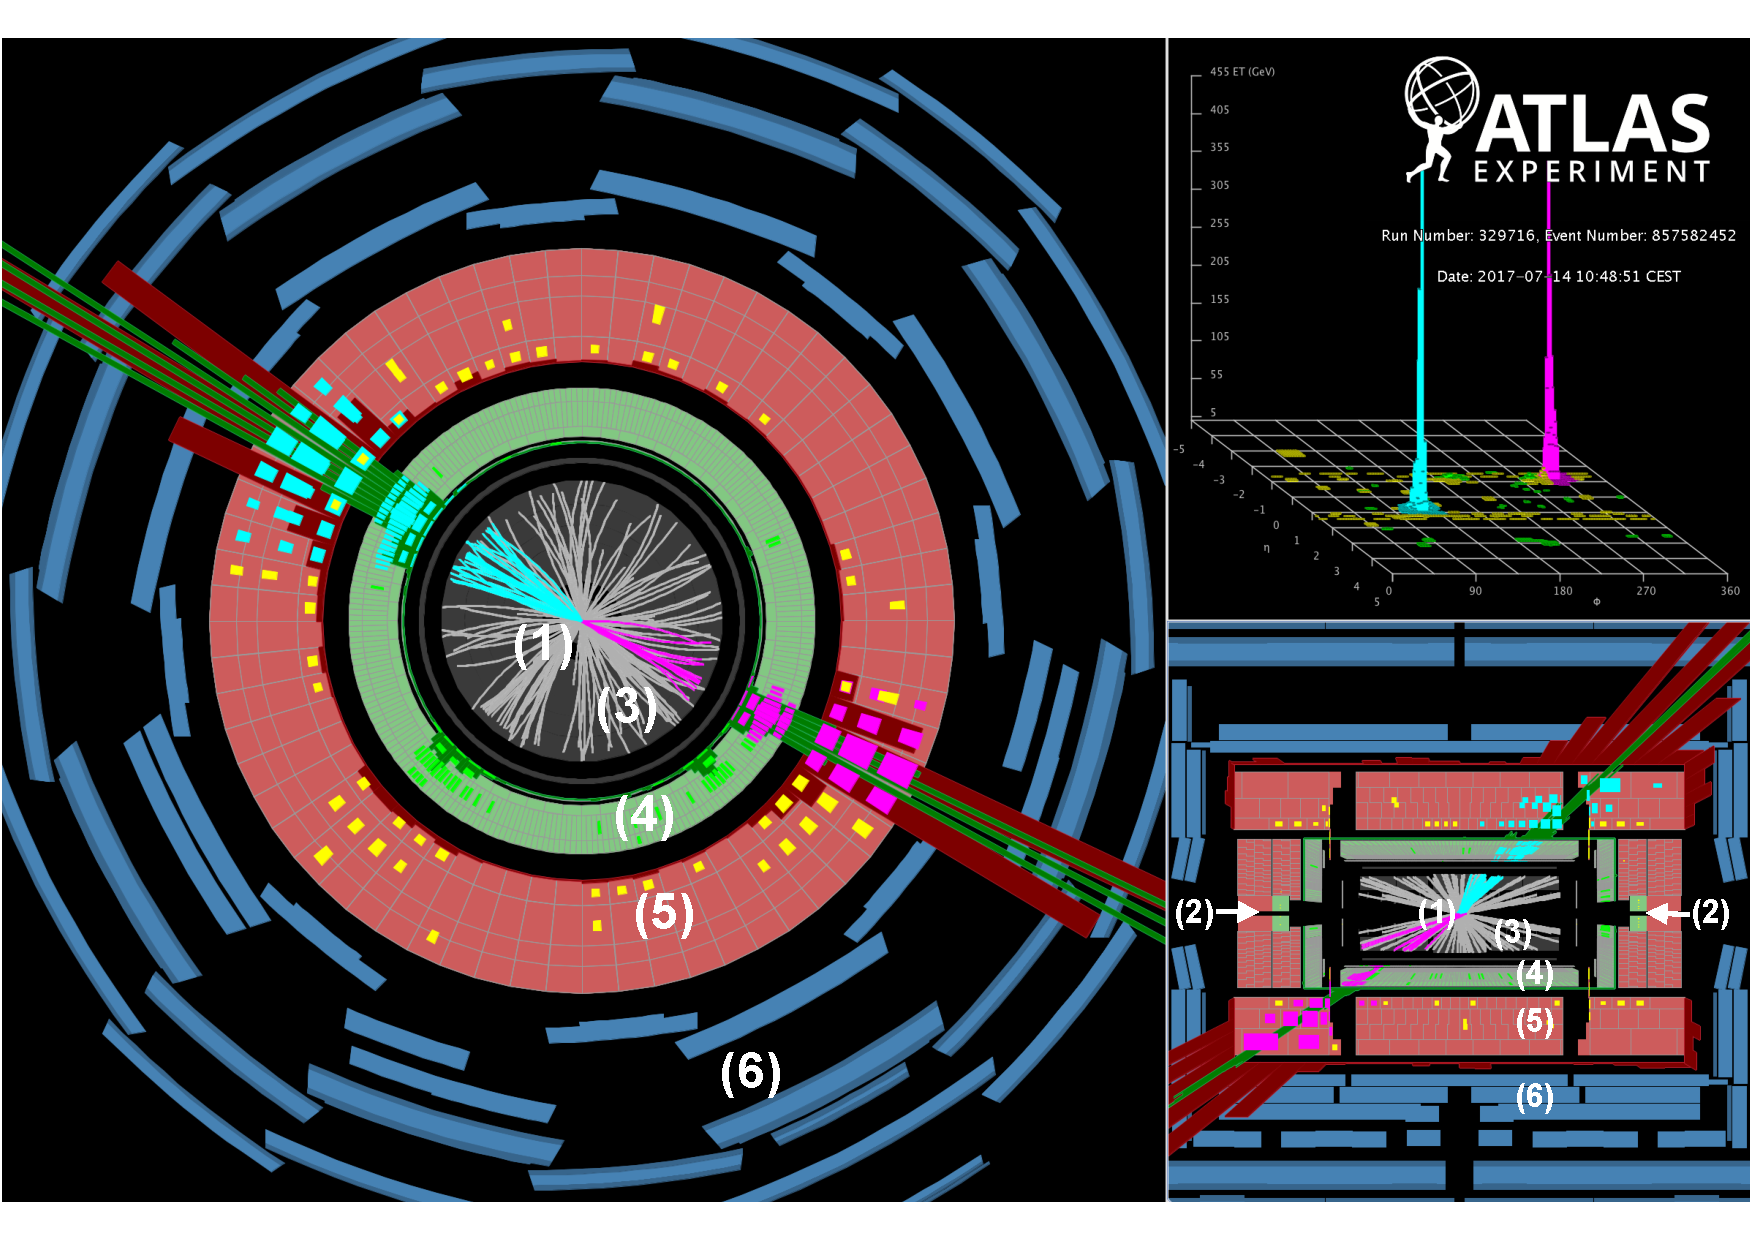
\includegraphics[width=0.90\textwidth]{figures/dijet_event_ATLAS.pdf}}
  \caption{
 Display of a dijet event recorded by ATLAS in proton-proton collisions at centre-of-mass energy 13~TeV. 
The two high-$p_t$ jets have both transverse momentum of 2.9~TeV and the dijet system exhibit an invariant mass of 9.3~TeV. 
The different panels correspond to the view of the event in the plane transverse to the beam direction (large figure on the left-hand side). The two smaller figures on the right-hand side show the calorimeter clusters transverse energies in the $(\eta,\phi)$ plane on the top and the longitudinal view of the event on the bottom. 
The numbers corresponds to different detectors components, as discussed in the text. 
%The figure has been taken and modified from~\cite{dijet-event}.
ATLAS Experiment~\copyright~2018 CERN.}
  \label{fig:detector}
\end{figure}

Multi-purpose detectors at the LHC are cylinder-shaped highly-complex
objects consisting of layers of different components, as depicted in
Fig.~\ref{fig:detector}, each component measuring a certain way a
particle can interact with the detector. Fig.~\ref{fig:detector} shows
a dijet event with an invariant mass of the two jets of $m_{jj} = 9.3$
TeV, measured by ATLAS and consists of three different images. In the
large image on the left the detector plane transverse to the beam axis
is shown. In the lower image on the right we see a lengthwise slice of
the ATLAS detector. The upper image on the right shows the energy
deposits of particles transverse to the beam axis in the so-called
{\it lego-plot} plane. In the lego plot the cylinder shape of the
detector is projected onto a 2-dimensional plane, consisting of the
variables $\eta \in (-\infty, \infty)$, the pseudo-rapidity, cf.\
Eq.~\eqref{eq:def-pseudo-rapidity}, and the azimuthal angle $\phi \in
[0,2 \pi]$.
% 
$\eta$ measures how forward a particle is emitted during the proton-proton interaction. 
Note the similarities between the pseudo-rapidity and the rapidity defined in Eq.~(\ref{eq:def-rapidity}): the two coincide for massless particles. 
%
Distances between two cells or particles $i$ and $j$ on the lego plane are measured via 
\begin{equation}
\Delta R_{ij}^{\text{(detector)}} = \sqrt{(\phi_i - \phi_j)^2 + (\eta_i -\eta_j)^2 }.
\label{eq:dr_eta}
\end{equation}
Note that the topoclusters are assumed massless, i.e. their rapidity equates their pseudo-rapidity. Thus, for detector cells the definitions of Eqs.~(\ref{eq:dr_eta}) and~(\ref{eq:DeltaR-def}) agree.
The different detector components are labelled in Fig.~\ref{fig:detector} in the following way:
\begin{itemize}
\item[(1)] Interaction point of the proton beams.
\item[(2)] The arrows indicate the direction of the particle beams. The proton beams are entering from either side of the detector and exit on the opposite side after crossing at the collision point.
\item[(3)] The innermost part of the ATLAS and CMS detectors consists of the tracking detectors which measure the momentum of charged particles. Strong magnetic fields bend the particles when traversing through the detectors. The way the tracks are bent is indicative of the particle's charge, mass and velocity.
\item[(4)] The electromagnetic calorimeter measures predominantly the energies of electrons and photons. Such particles are stopped and induce a cascade of particles, \emph{a shower}, in the calorimeter. Charged particles can be discriminated from photons by the presence or absence of tracks in the tracking detectors. Cell sizes for this calorimeter vary between the central and forward direction of the detector. In the central part they are roughly $(0.025 \times 0.025)$ in the $\phi-\eta$ plane.
\item[(5)] The hadronic calorimeter measures the energies of hadronic particles, e.g. protons and neutrons. As in the case of the electromagnetic calorimeter, charged hadrons can be discriminated from neutral ones due to their energy loss in the tracking detectors. The cells that make the hadronic calorimeter have in the central region of the detector a size of roughly $(0.1 \times 0.1)$ in the $\phi-\eta$ plane.
\item[(6)] The most outer layer of the detector is the muon spectrometer. Muons, produced with characteristic LHC energies, are weakly interacting with the detector material and are consequently not stopped. However, they may leave tracks in the tracking system, undergo energy loss in the electromagnetic and hadronic calorimeter and may eventually interact with the muon spectrometer. 
\end{itemize}

\begin{figure}
  \centerline{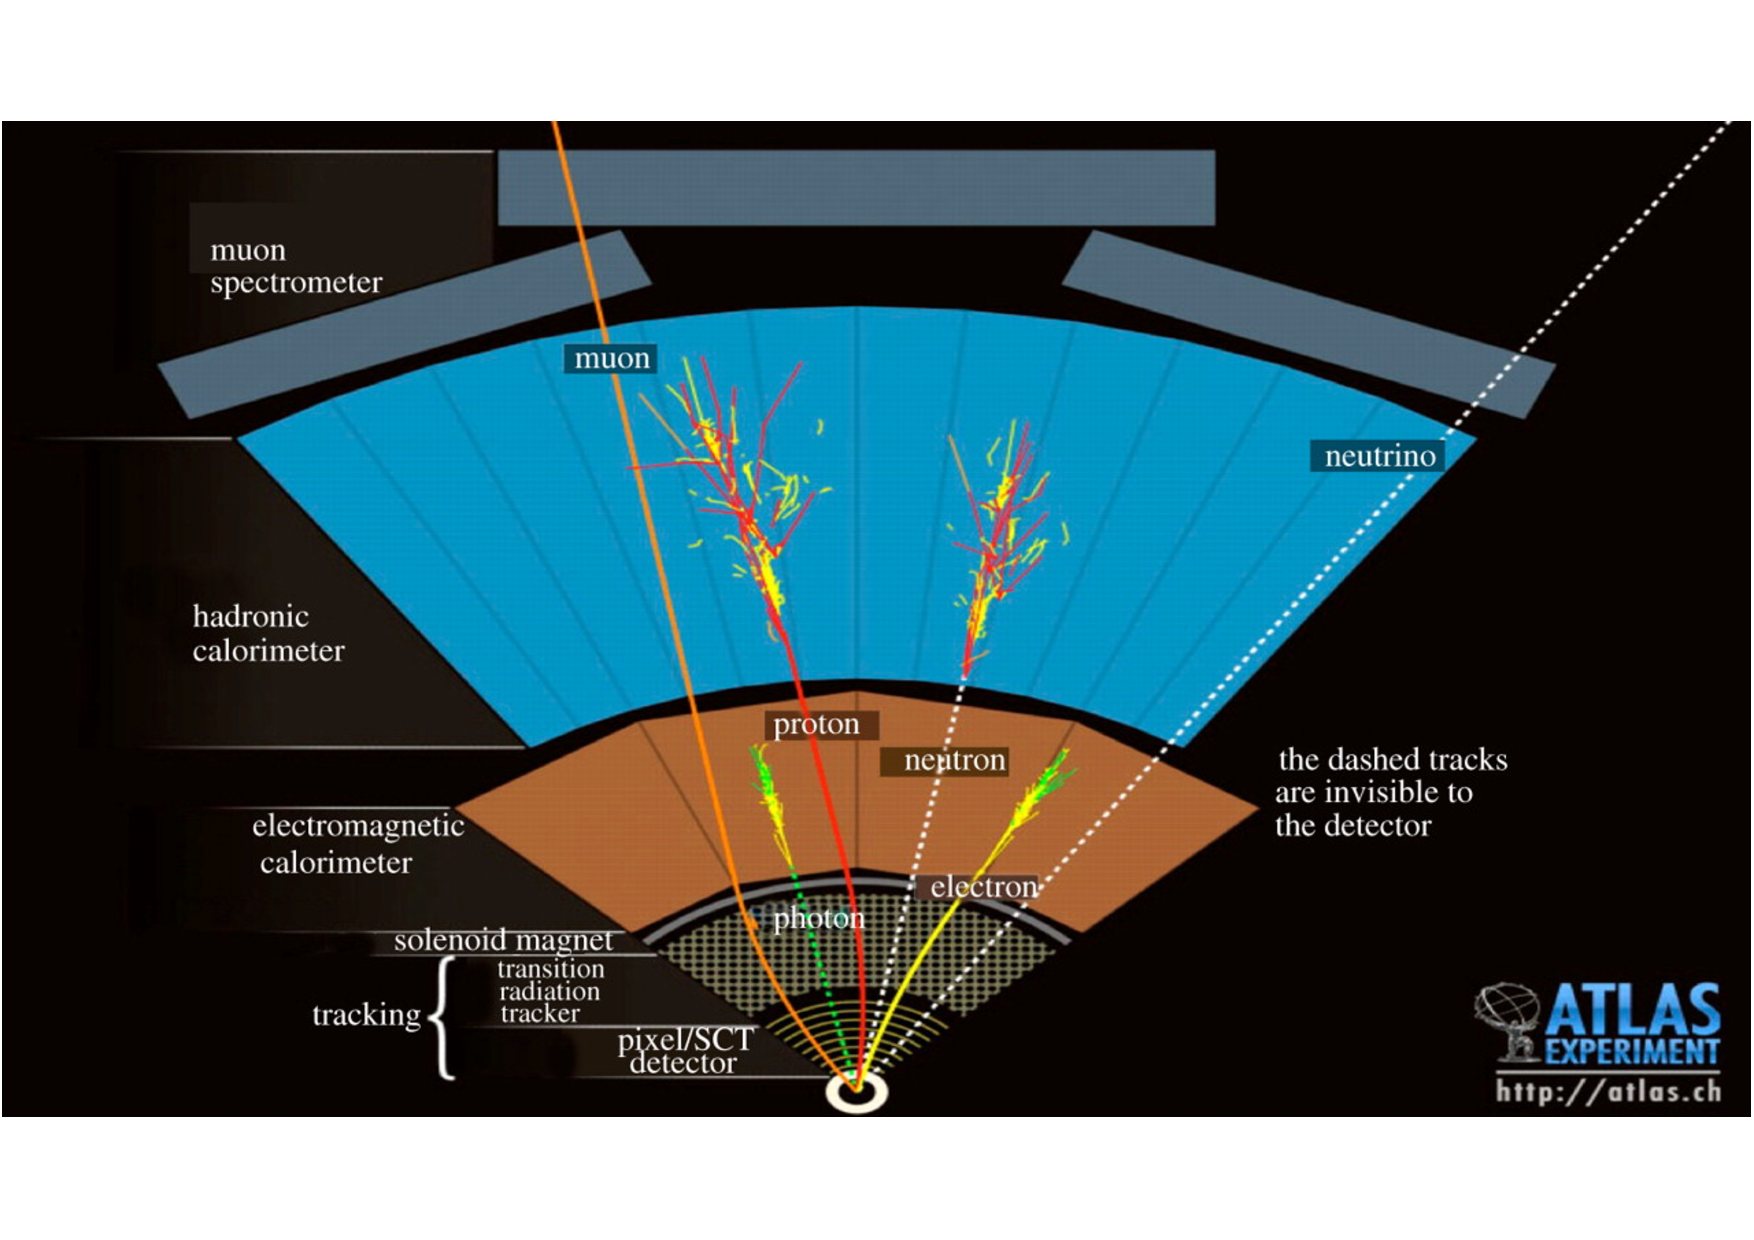
\includegraphics[width=0.95\textwidth]{figures/detector_large.pdf}}
  \caption{Schematic depiction of a multi-purpose detector, here ATLAS. The picture illustrates how different particles interact with the various layers of the detector.  
  ATLAS Experiment~\copyright~2018 CERN.
%  The figure has been taken from Ref.~\cite{Kourkoumelis:2013vpa}).
}
  \label{fig:interaction}
\end{figure}


In Fig.~\ref{fig:interaction} we show a segment of a slice of the transverse plane and how classes of particles interact with the individual detector components. For each high-energy Standard Model event we expect of $\mathcal{O}(500)$ resulting particles, which we can classify into photons, charged leptons, neutral and charged hadrons and non-interacting particles, i.e.\ neutrinos. In a typical proton-proton collision, about 65\% of the jet energy is carried by charged particles, 25\% by photons, produced mainly from $\pi_0$ decays, and only 10\% by neutral hadrons (mostly neutrons and $K_{L} $) \cite{CMS:2010byl, CMS:2010eua}. However, these fractions can vary significantly from event to event.

 
Charged particles loose energy when traversing the detector material in various ways. One mechanism is ionisation and excitation interactions with the detector material, e.g. $\mu^- + \mathrm{atom} \to \mathrm{atom}^* + \mu^- \to \mathrm{atom} + \gamma + \mu^-$, where their energy loss per distance is governed by the Bethe equation \cite{Tanabashi:2018oca}. Further mechanisms for charged particles to interact with the detector material are {\it bremsstrahlung}, {\it direct electron-pair production} and {\it photonuclear interactions
}. 
Photons interact with the detector material through {\it photoelectric effect}, {\it Compton scattering} and {\it electron-pair production}. The latter being dominant for $E_\gamma \gg 1$ MeV.
In the case of hadron-detector interactions, we are dealing mostly with inelastic processes, where secondary strongly interacting particles are produced in the collision.

\vspace{0.3cm}

\begin{wrapfigure}{R}{0.5\textwidth}
 \centering
  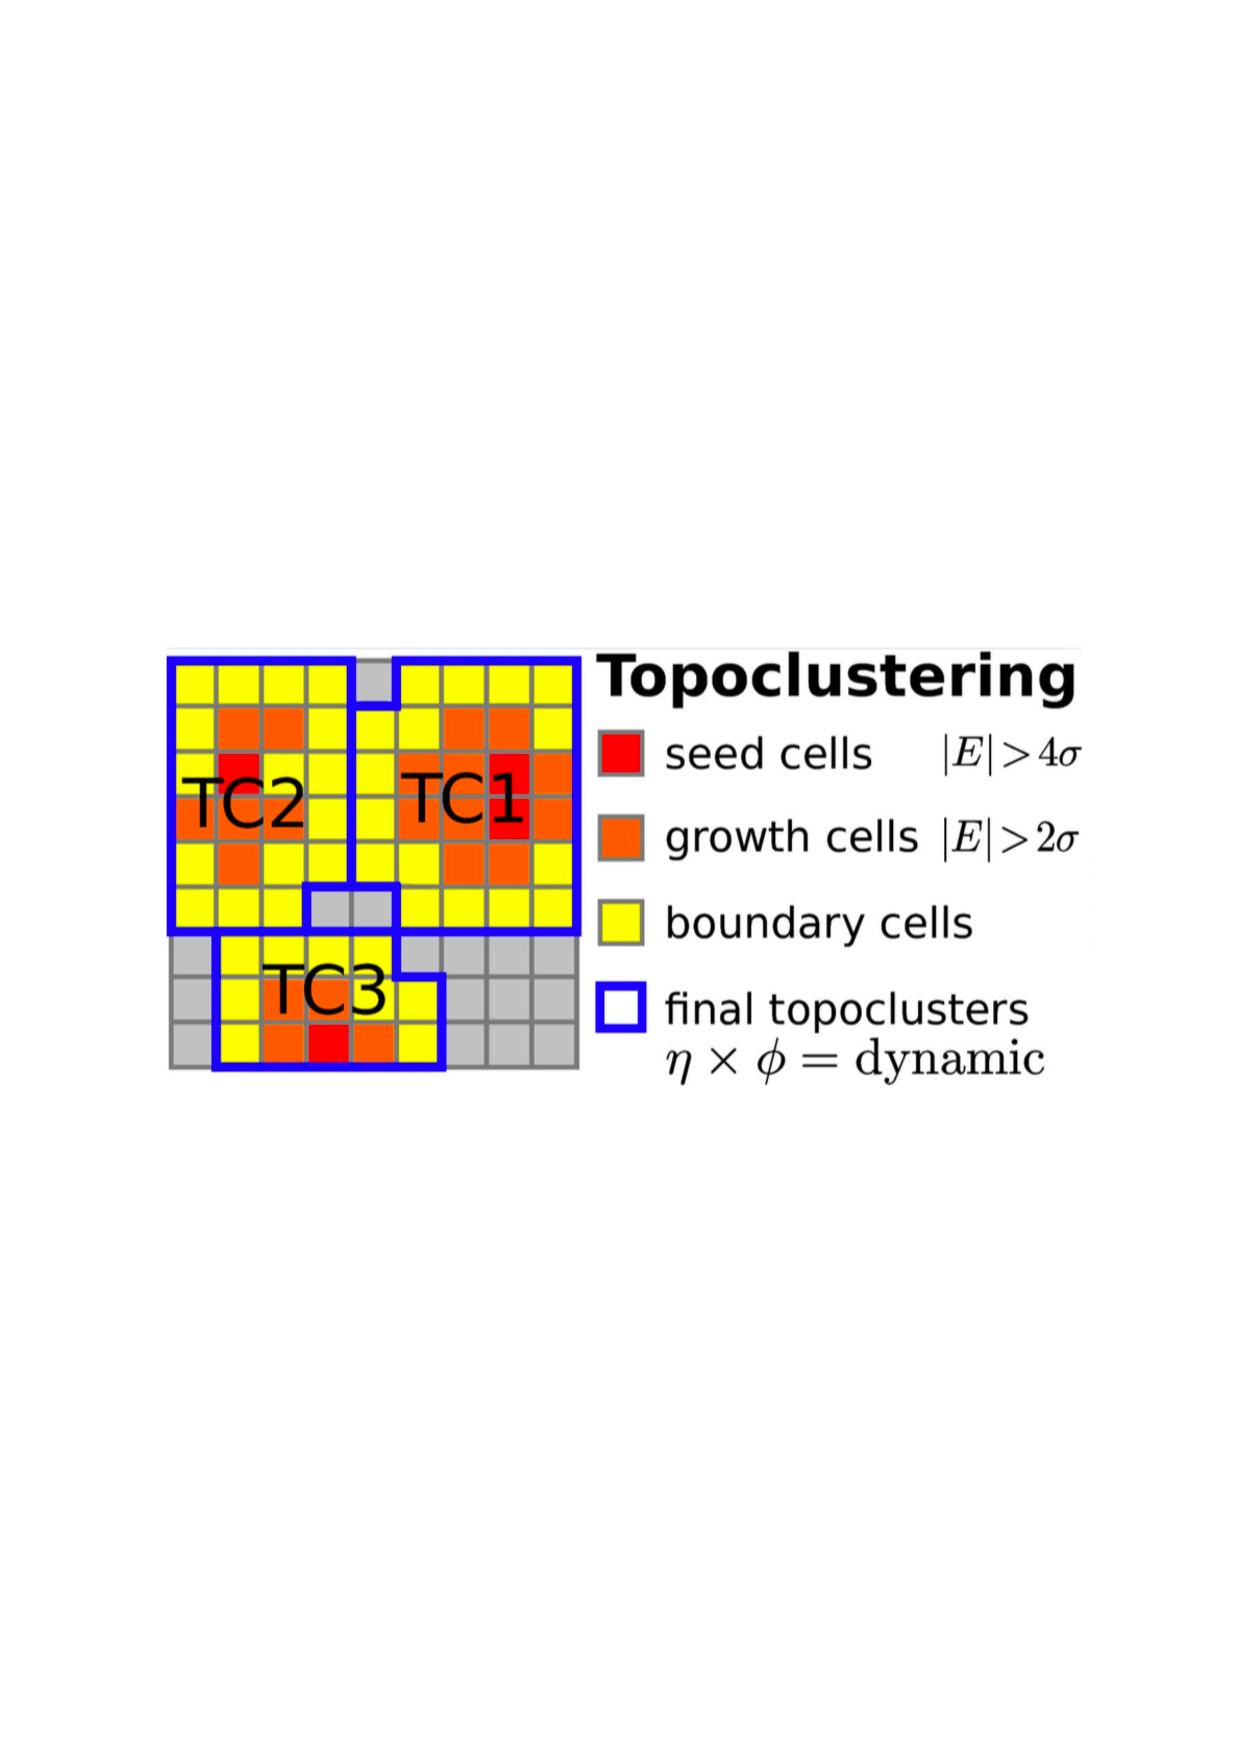
\includegraphics[width=0.5\textwidth]{figures/topocluster.pdf}
  \caption{The figure shows how calorimetric information is used by ATLAS to construct jet constituents (taken from~\cite{boosttalk}).}
  \label{fig:topoclusters}
\end{wrapfigure}

Information gathered from the detector components (3)-(6) allow to
obtain a global picture of the particles produced in the
event. However, particles are not directly used as input to construct
jets using the algorithms previously discussed. ATLAS and CMS use
different approaches to construct jet constituents. The former is
using topological clusters, or, in short, topoclusters, which are
mainly based on calorimeter objects, while the latter use so-called
particle flow objects, which combine information from the tracker and
the calorimeter to build a coherent single object.\footnote{Note that
  ATLAS is moving to using a particle flow approach as well.} The
benefit of using calorimeter objects is a good calibration of the
energy component of the topoclusters. On the other hand, the cell size
of the hadronic calorimeter is $0.1 \times 0.1$ in $(\eta, \phi)$ and
topological cell clusters are formed around seed cells with an energy
$|E_\mathrm{cell}|$ at least $4 \sigma$ above the noise by adding the
neighbouring cells with $|E_\mathrm{cell}|$ at least $2\sigma$ above
the noise, and then all surrounding cells \cite{Aad:2012vm}, see
Fig.~\ref{fig:topoclusters}. The minimal transverse size for a cluster
of hadronic calorimeter cells is therefore $0.3 \times 0.3$ and is
reached if all significant activity is concentrated in one cell. Two
energy depositions leave distinguishable clusters if each one hits
only a single cell and their individual axes are separated by at least
$\Delta R = 0.2$, so that there is one empty cell between the two seed
cells. In the context of this bbok, it means that if important
characteristics of the substructure in a jet are so close that it does
not leave separate clusters in the jet, it is impossible to resolve
it. This leaves a residual lower granularity scale when using
topocluster as fundamental objects to form jets. Thus, in particular
when a fine-grained substructure in the jet is of importance, e.g. in
the reconstruction of highly boosted resonances, the benefit of
particle flow objects is widely appreciated across both multi-purpose
experiments.





Focusing exclusively on the tracking detectors when reconstructing jets is an even more radical approach to optimising the spatial resolution of a final state. Tracking detectors can reconstruct the trajectories of a charged particles, which carry $\sim 65\%$ of the final state's energy, and can specify the direction of the particle at any point of the trajectory with a precision much better than the granularity of the calorimeter. For example, the angular resolution of the ATLAS inner tracking detector for charged particles with $p_T = 10$ GeV and $\eta  = 0.25$ is $\sim 10^{-3}$ in $\eta$ and $\sim 0.3$ mrad in $\phi$ \cite{Aad:2008zzm} with a reconstruction efficiency of $> 78\%$ for tracks of charged particles with $p_T > 500$ MeV \cite{Aad:2010ac}. Further, the momentum resolution for charged pions is 4\% for momenta $|p| < 10$ GeV, rising to 18\% at $|p| = 100$ GeV \cite{Aad:2008zzm}.
%
Note that, generally speaking, the energy resolution tends to degrade
with energy in for calorimeters, but improves with energy for trackers.


%  LocalWords:  topoclusters Eq eq lego Eqs


\section{Implementation}\label{sec:jetdefs-implementation}
\begin{figure}
  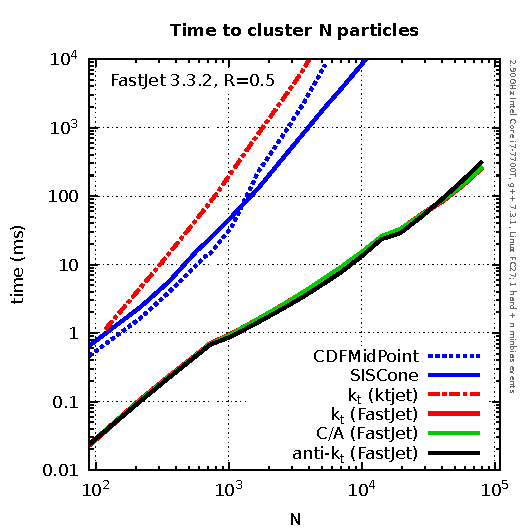
\includegraphics[width=0.53\textwidth]{figures/fastjet-timings.pdf}
  \hspace*{0.4cm}
  \begin{minipage}[b]{0.38\textwidth}
    \caption{Average clustering time as a function of the event
      multiplicity $N$, obtained with the FastJet implementation of
      several representative algorithms.}\label{fig:fastjet-timings}
    \vspace*{1.4cm}
  \end{minipage}  
\end{figure}


Most of the practical applications of jets use numerical inputs,
either from (fixed-order or parton-shower) Monte Carlo simulations, or
directly from experimental data. It is therefore important to have a
numerical implementation of the jet algorithms.
%
Furthermore, this implementation needs to be fast enough for practical
usability in an experimental (and, to a lesser extent, theoretical)
context.
%
Currently, the standard package for jet clustering is
{\tt{FastJet}}~\cite{Cacciari:2005hq,Cacciari:2011ma},\footnote{See
  also \url{http://fastjet.fr}.} used by both the experimental and
theoretical communities at the LHC. It provides a native
implementation of all the recombination algorithms introduced in
Sec.~\ref{sec:jetalgs-recombination} and plugins for a series of
other jet algorithms, including the cone algorithms discussed in
Sec.~\ref{sec:jetalgs-cone}.
%
As an illustration, we show in Fig.~\ref{fig:fastjet-timings} the
average time it takes to cluster an event with $N$ particles for a few
representative algorithms.
%
For the specific case of the $k_t$ algorithm, we show the timings for
two different implementations: the initial {\tt{ktjet}}
implementation~\cite{Butterworth:2002xg} available at the time of the
Tevatron and deemed too slow, and the {\tt{FastJet}} implementation
which is faster by 2-3 orders of magnitude in the region relevant for
phenomenology (around a few thousands particles).
%
Regarding cone algorithms, this plot shows that
infrared-and-collinear SISCone has clustering times similar to the
unsafe MidPoint.\footnote{MidPoint has here been used with a seed
  threshold of 1~GeV. Without a seed threshold, it would be slower by
  about an order of magnitude.}
%
Finally, if one keeps in mind that in practical (trigger-level) jet
reconstruction at the LHC, one has a few tens of milliseconds for
clustering, Fig.~\ref{fig:fastjet-timings} shows that the
recombination algorithms (and their {\tt{FastJet}} implementation) are
currently clearly preferred.

%% GS helper for auctex
%%% Local Variables:
%%% mode: latex
%%% TeX-master: "notes"
%%% End:
%  LocalWords:  WTA Snowmass kinematically iB ij JetClu ktjet
%  LocalWords:  MidPoint
